\usetikzlibrary{decorations.pathmorphing}
\usetikzlibrary{decorations.markings}
\usetikzlibrary{decorations.pathmorphing}
\usetikzlibrary{arrows}
\usetikzlibrary{automata}
\usetikzlibrary{decorations.markings}
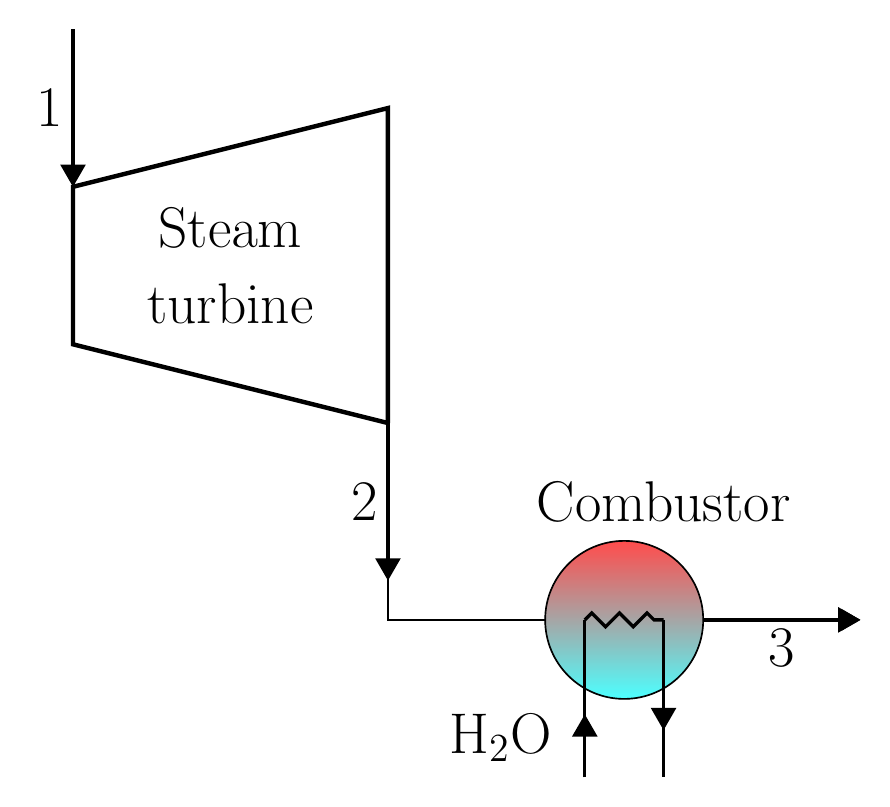
\begin{tikzpicture}[>=triangle 60]

\tikzset{->-/.style={decoration={
  markings,
  mark=at position #1 with {\arrow{>}}},postaction={decorate}}}
  
\tikzset{-<-/.style={decoration={
  markings,
  mark=at position #1 with {\arrow{<}}},postaction={decorate}}}

%trapezio
\draw[ultra thick] (5.5,0)--(1.5,1)--(1.5,3)--(5.5,4)--(5.5,0);

%steam turbine
\node [anchor=center,align=center] at (3.5,2) {\huge Steam\\\\ \huge turbine}; 

%arrow 2
\draw[very thick,->] (5.5,0)--(5.5,-2);
\node [anchor=east] at (5.5,-1) {\huge $2$}; 

%arrow 1
\draw[very thick,<-] (1.5,3)--(1.5,5);
\node [anchor=east] at (1.5,4) {\huge $1$}; 

\draw[thick,->] (5.5,0)--(5.5,-2.5)--(11.5,-2.5);


%combustor
\draw[fill=white,thick,draw=black] (8.5,-2.5) circle(1);
%\draw[thick] (8,-4.5)--(8,-2.5)--(9,-2.5)--(9,-4.5);

%combustor fill
\filldraw[top color=red!70,bottom color=cyan!70] (8.5,-2.5) circle (1); 
%\draw[thick,fill=red!40] (9.5,-2.5) arc (0:180:1); 
%\draw[thick,fill=blue!40] (9.5,-2.5) arc (0:-180:1); 

\draw[->-=0.4,very thick] (8,-4.5)--(8,-2.5);
\draw[very thick,decorate,decoration=zigzag] (8,-2.5)--(9,-2.5);
\draw[->-=0.7,very thick] (9,-2.5)--(9,-4.5);

\node [anchor=east] at (7.7,-4) {\huge H$_2$O}; 

%combustor text
\node [anchor=center,align=center] at (9,-1) {\huge Combustor}; 

%arrow 3
\draw[very thick,<-] (11.5,-2.5)--(9.5,-2.5);
\node [anchor=north] at (10.5,-2.5) {\huge $3$}; 

\end{tikzpicture}